\chapter{Performance and Limitations}

It is important to know the capabilities of the airplane. It is also important to note how they change.

The Lance in particular has a huge variation in operating weight and center of gravity. A nose loaded, light Lance is practically a different airplane from a tail loaded, heavy Lance. It's important to explore the envelope of the plane in flight. But first, it's important to understand the envelope on the ground.

This chapter references the Lance's POH heavily. It is here: \url{https://tinyurl.com/n36262poh}.


\section{The Power Curve}

We're engineers! We want a rigorous definition of all of the above speeds and their variation.

John S. Denker in ``See How It Flies'' has the most beautiful power curve diagram I've seen. It ties together the three major regimes of flight - normal, slow, and stalled - in one simple diagram. To me it is more clear than the classic diagram that plots lift, drag, and their ratio.

Here is Denker's power curve at idle power.

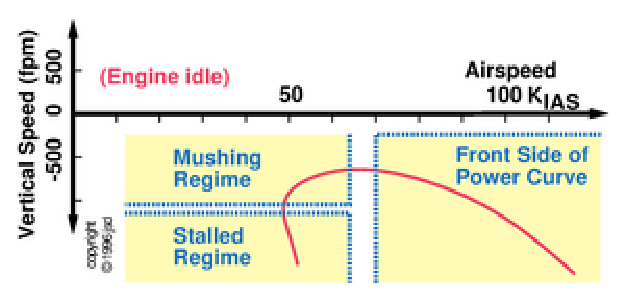
\includegraphics[width=\linewidth]{power-curve-regimes}

We plot airspeed on the X axis and vertical speed on the Y axis. The curve is decidedly not a function: it doubles back on itself. But we can piecewise define it as three functions. We draw a vertical tangent line on the left edge and a horizontal tangent line at the top edge. We'll talk about those tangent points later, they're important. But they define the limits of our three regimes of interest: normal, slow, and stalled. Or as Denker calls them, front side, mushing, and stalled.

Of course, this is at idle power. Since power makes us climb, but the power curve represents a fixed relationship between adjacent speeds that is always the same shape for the airplane, setting power moves the curve up or down. Denker wrote this for a fixed pitch prop, we can instead imagine 55, 65, and 75 percent power.

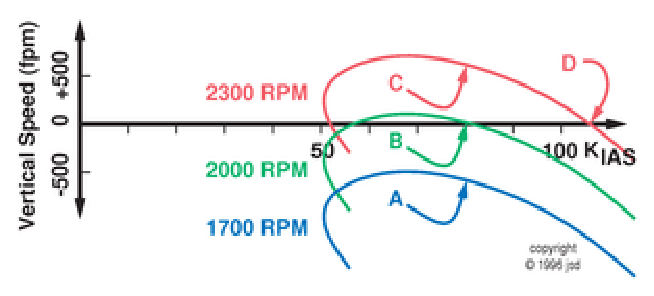
\includegraphics[width=\linewidth]{three-power}

The one gotcha with this explanation of the power curve is that it doesn't really explain what the flaps do directly. But we can derive it. Flaps change the shape of the airfoil and give us more lift in exchange for more drag. Low flap settings give us mostly more lift, high flap settings give us mostly more drag. More lift means moving the curve up. More drag meand moving the curve to the left.

\section{Speed Definitions}

Now that we've built a rigorous framework for describing airplane behavior using the power curve mode, we can go ahead and define some speeds. The following speeds are appropriate for a complex single engine airplane. We do quote the Lance's POH here heavily but I find the POH definitions sorely lacking.

$V_S$ or $V_{S0}$ are the stalling speeds in the cruise or clean configuration: gear up, flaps up. This is the leftmost point on the power curve, the barrier between the stalled and mushing regimes. From the Lance's POH: ``stalling speed, or the minimum steady flight speed at which the airplane is controllable.''

$V_{S1}$ is the stalling speed in the landing or dirty configuration: gear down, flaps down. Since extending the flaps moves the power curve to the left, stalling speed is lowered.

$V_R$ is the rotation speed. Denker suggests a few knots below $V_Y$ unless specifically doing a short or soft field takeoff. In those cases I'd lift off right at or around $V_X$.

$V_X$ is the best \emph{angle} of climb speed, which we use to clear an obstacle. Denker draws a tangent from the origin of his performance curve axes to the power curve, the point of intersection is $V_X$. That speed will get slower if the power curve moves up (more lift) or to the left (more drag).

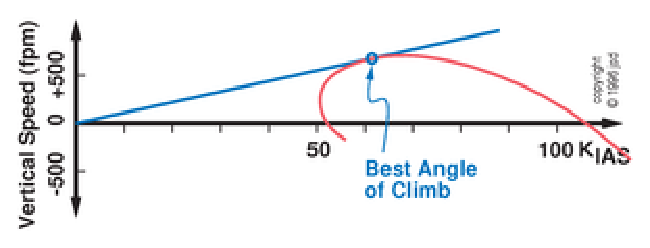
\includegraphics[width=\linewidth]{vx}

$V_Y$ is the best \emph{rate} of climb speed, which we use to gain altitude quickly. It corresponds to the maximum lift over drag speed, meaning, the most efficient point of operation. The maximum endurance speed is usually not far from this value. Denker draws this at the top of the power curve, or rather, where a horizontal line would be tangent to the curve. This does change with weight but as Denker points out the power curve is pretty flat here.

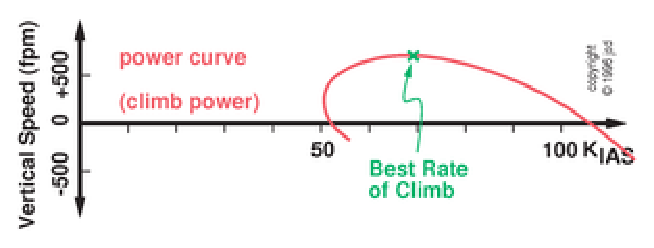
\includegraphics[width=\linewidth]{vy}

$V_G$ is the best glide speed. $V_Y$ is a reasonable guess.

$V_{FO}$ is the flap operation speed. We don't have a specific one for the Lance.

$V_{FE}$ is the flap extension speed. This is the speed at which the flaps may be extended. From the POH: ``the highest speed permissible with wing flaps in a prescribed extended position.''

$V_A$ is the maneuvering speed. It is ``the maximum speed at which application of full available aerodynamic control will not overstress the airplane.'' I talk about $V_A$ in a later chapter, but realize that it depends on weight, and tests \emph{a single control's full deflection at once}. Putting multiple controls to full deflection may overstress the airframe.

$V_{LO}$ is the landing gear operation (retraction) speed. This is the maximum speed at which the landing gear may be safely extended or retracted.

$V_{LE}$ is the landing gear extended speed. It is ``the maximum speed at which an aircraft can be safely flown with the landing gear extended.''

$V_{NO}$ is the ``normal operating'' speed. ``Maximum Structural Cruising Speed is the speed that should not be exceeded except in smooth air and then only with caution.''

$V_{NE}$ is the never exceed speed. Operations past this speed are likely to cause structural damage to the aircraft.

\section{Lift and Weight}

Recall the lift equation:

\begin{equation}
L = \frac{1}{2} \rho V^2 C_L S
\end{equation}

, where $\rho$ is the density of the air, $V$ is velocity, $C_L$ is the coefficient of lift and $S$ is the surface area of the airfoil.

That $V^2$ term is key, Lift is proportional to the \emph{square} of velocity. So what happens if we halve the weight, and thus, the needed lift? Well, it would drop by the square root of a half, which happens to be $\frac{\sqrt{2}}{2} \approx 0.707\ldots$ which is about 29 percent. At three-quarters weight, it drops by the square root of three quarters, which is $\frac{\sqrt{3}}{2} \approx 0.866\ldots$ which is about 13 percent.

Denker points out that the entire power curve shifts up and to the right, with both power off and power on. He even points out a Cherokee Six as a specific example of this - how interesting!

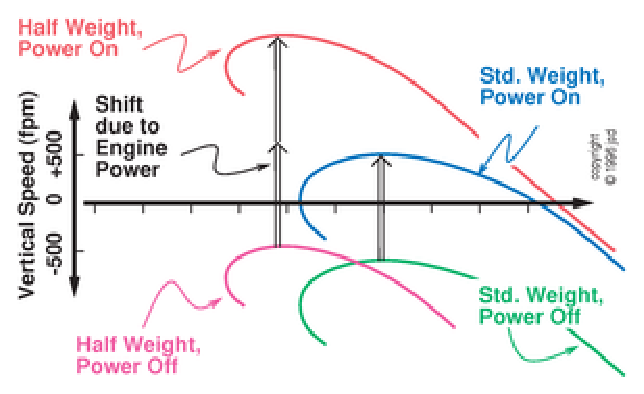
\includegraphics[width=\linewidth]{light-power}

The procedure to derive this curve is as follows:

\begin{enumerate}
\item Scale the entire standard weight, power off curve by the reduction factor. It will move up (since vertical speeds are chopped - a light airplane doesn't sink as much) and to the left (since airspeeds go down - a light airplane has a lower stalling speed).
\item Shift the curve up for power. Realize that, since the airplane is lighter, the curve will shift by a greater amount.
\end{enumerate}


\section{V Speeds for the Lance}

The Lance's POH defines a number of speeds. These speeds are commonly defined for single engine airplanes.

In this section, we explore the Lance's V speeds. For each V speed, we consider the definition of the speed, what it means operationally, and how it varies with respect to aircraft weight, aircraft loading (nose or tail heavy), density altitude, aircraft configuration (flaps, landing gear), and aircrat attitude.

The beginning of Section 4 of the POH provides many of these figures.

Recall the weights and speeds variation formula, which we can derive from two different values of the lift formula. It is written here for stall speed but applies to many speeds in this section.

\begin{equation}
V_S' = V_S \sqrt{\frac{New\ Weight}{Old\ Weight}}
\end{equation}

We can use this formula to calculate different speeds for a few different weights. I'll show values for 3600 lbs (max gross), 3200 lbs, 2800 lbs, 2400 lbs, and the airplane's minimum weight (with third row seats removed) of 2151 lbs as per the most recent POH.

Here is a cheat sheet with all the V speeds at max gross weight.

\begin{figure}
\begin{center}
\begin{tabular}{ |c|c|c| }
    \hline
    $V$ Speed & Value (KIAS) & Marking\\
    \hline
    \hline
     $V_{SO}$ &  52 & Bottom of White Arc \\
     $V_S$    &  53 & Bottom of Green Arc \\
    \hline
     $V_R$    &  87 & None \\
    \hline
     $V_X$    &  68-87 & None \\
     $V_Y$    &  92    & None \\
    \hline
     $V_{FE}$ &  109 & Top of White Arc \\
     $V_A$    &  132 & Placard \\
    \hline
     $V_{LO}$ &  106 & Placard \\
     $V_{LE}$ &  129 & Placard \\
    \hline
     $V_{NO}$ &  150 & Bottom of Yellow Arc \\
     $V_{NE}$ &  191 & Red Line \\
    \hline
\end{tabular}
\end{center}
\caption{V Speeds - P32T}
\label{fig:VSpeedsP32T}
\end{figure}

\subsection{$V_{S}$ - Stalling Speed}

52-53 KIAS.

Variation Chart: see Figure ~\ref{fig:StallSpeedsP32T}.

\begin{figure}
\begin{center}
\begin{tabular}{ |c|c| }
    \hline
    Weight & Stalling Speed \\
    (pounds) & (KIAS) \\
    \hline
     3600 &  53 \\
     3200 &  50 \\
    \hline
     2800 &  47 \\
     2400 &  43 \\
    \hline
     2151 &  41 \\
    \hline
\end{tabular}
\end{center}
\caption{Stalling Speed Weight Variance - P32T}
\label{fig:StallSpeedsP32T}
\end{figure}


\begin{itemize}
\item Markings: Bottom of green arc for flaps up. Bottom of white arc for flaps down.
\item Weight: a heavier airplane will require a higher angle of attack to fly and thus will have a higher stalling speed. A lighter airplane will have a lower stalling speed.
\item Loading: a nose heavy airplane will have a higher stalling speed due to the high angle of attack required to keep the nose flying. Conversely, an aft loaded airplane will have a lower stalling speed. But according to Denker the effect is relatively small.
\item Density Altitude: In thinner air, there is a greater discrepancy between indicated and calibrated airspeed. The airplane will stall at the same indicated airspeed but a higher true airspeed.  
\item Configuration: Changing the shape of the wings by deploying flaps changes the effective angle of attack. Deploying flaps will usually make the stall speed decrease.
\item Attitude: Stalling speed increases in a turn since we are using a larger component of our lift vector to keep the airplane aloft. In turbulence, the angle of incidence may vary, leading to an earlier stall because the relocation of the relative wind causes us to exceed critical angle of attack earlier. 
\end{itemize}


\subsection{$V_{NE}$ - Never Exceed Speed}

191 KIAS or 189 KCAS

Variation Chart: None. This is an absolute value based on aerodynamic pressure, measured with the pitot tube. The wings and tail can crumple at any weight.

\begin{itemize}
\item Markings: Top of the yellow arc on the airspeed indicator. Red line on same indicator.
\item Weight: No factor.
\item Loading: No factor.
\item Density Altitude: Will occur at a higher true airspeed, but same indicated airspeed, at high density altitude.
\item Configuration: TODO
\item Attitude: TODO
\end{itemize}

\subsection{$V_{NO}$ - Maximum Structural Cruising Speed}

150 KIAS or 150 KCAS

Variation Chart: None. This is an absolute value based on aerodynamic pressure, measured with the pitot tube. The wings and tail can crumple at speeds beyond this in turbulence due to momentary increases in load factor. Operations in this region, including descents, are approved in smooth air. Proceed with caution!

\begin{itemize}
\item Markings: TODO
\item Weight: TODO
\item Loading: TODO
\item Density Altitude: TODO
\item Configuration: TODO
\item Attitude: TODO
\end{itemize}

\subsection{$V_A$ - Design Maneuvering Speed}

132 KIAS or KCAS at max gross weight. Also ``Turbulent Air Operating Speed''.

Variation Chart: Per POH, use linear interpolation to get $V_A$ at various weights. See Figure ~\ref{fig:MAneuveringSpeedsP32T}.

\begin{figure}
\begin{center}
\begin{tabular}{ |c|c| }
    \hline
    Gross Weight & Maneuvering Speed \\
    (pounds) & (KIAS) \\
    \hline
     3600 &  132 \\
     3400 &  129 \\
    \hline
     3200 &  126 \\
     3000 &  123 \\
    \hline
     2800 &  120 \\
     2600 &  117 \\
    \hline
     2400 &  115 \\
     2151 &  112 \\
    \hline
\end{tabular}
\end{center}
\caption{Maneivering Speed Weight Variance - P32T}
\label{fig:ManeuveringSpeedsP32T}
\end{figure}

\begin{itemize}
\item Markings: Placarded for max gross weight.
\item Weight: TODO
\item Loading: TODO
\item Density Altitude: TODO
\item Configuration: TODO
\item Attitude: TODO
\end{itemize}

\subsection{$V_{FE}$ - Maximum Flaps Extended Speed}

109 KIAS or KCAS

Variation Chart: None. This is a structural limitation.

\begin{itemize}
\item Markings: TODO
\item Weight: TODO
\item Loading: TODO
\item Density Altitude: TODO
\item Configuration: TODO
\item Attitude: TODO
\end{itemize}

\subsection{Maximum Landing Gear Extension Speed}

129 KIAS or 130 KCAS

Variation Chart: None. This is a structural limitation.

\begin{itemize}
\item Markings: TODO
\item Weight: TODO
\item Loading: TODO
\item Density Altitude: TODO
\item Configuration: TODO
\item Attitude: TODO
\end{itemize}

\subsection{Maximum Landing Gear Retraction Speed}

106 KIAS or 109 KCAS

Variation Chart: None. This is a structural limitation.

\begin{itemize}
\item Markings: TODO
\item Weight: TODO
\item Loading: TODO
\item Density Altitude: TODO
\item Configuration: TODO
\item Attitude: TODO
\end{itemize}

\subsection{$V_{LE}$ - Maximum Landing Gear Extended Speed}

129 KIAS or 130 KCAS

Variation Chart: None. This is a structural limitation.

\begin{itemize}
\item Markings: TODO
\item Weight: TODO
\item Loading: TODO
\item Density Altitude: TODO
\item Configuration: TODO
\item Attitude: TODO
\end{itemize}

\subsection{Caution Range - Yellow Arc}

150 KIAS to 191 KIAS

Variation Chart: None. See prior discussion of $V_{NO}$.

\begin{itemize}
\item Markings: TODO
\item Weight: TODO
\item Loading: TODO
\item Density Altitude: TODO
\item Configuration: TODO
\item Attitude: TODO
\end{itemize}

\subsection{$V_Y$ - Best Rate of Climb Speed}

87 KIAS (gear down, flaps up) to 92 KIAS (gear up, flaps up)

Variation Chart: Yes. As this is a speed derived from the power curve, it is subject to translations and scalings of the power curve based on gross weight and configuration. See Figure ~\ref{fig:VYCleanP32T} for the clean configuration and ~\ref{fig:VYDirtyP32T} for the dirty configuration. I consider these speeds to be optimistic and generally add 2-3 knots.

\begin{figure}
\begin{center}
\begin{tabular}{ |c|c| }
    \hline
    Weight & Stalling Speed \\
    (pounds) & (KIAS) \\
    \hline
     3600 &  92 \\
     3200 &  87 \\
    \hline
     2800 &  81 \\
     2400 &  75 \\
    \hline
     2151 &  71 \\
    \hline
\end{tabular}
\end{center}
\caption{Best Rate of Climb Speed Weight Variance, Clean - P32T}
\label{fig:VYCleanP32T}
\end{figure}

\begin{figure}
\begin{center}
\begin{tabular}{ |c|c| }
    \hline
    Weight & Stalling Speed \\
    (pounds) & (KIAS) \\
    \hline
     3600 &  87 \\
     3200 &  82 \\
    \hline
     2800 &  77 \\
     2400 &  71 \\
    \hline
     2151 &  67 \\
    \hline
\end{tabular}
\end{center}
\caption{Best Rate of Climb Speed Weight Variance, Dirty - P32T}
\label{fig:VYDirtyP32T}
\end{figure}

\begin{itemize}
\item Markings: TODO
\item Weight: TODO
\item Loading: TODO
\item Density Altitude: TODO
\item Configuration: TODO
\item Attitude: TODO
\end{itemize}

\subsection{$V_X$ - Best Angle of Climb Speed}

68 KIAS (gear down, flaps up) to 87 KIAS (gear up, flaps up)

Variation Chart: Yes. As this is a speed derived from the power curve, it is subject to translations and scalings of the power curve based on gross weight and configuration. See Figure ~\ref{fig:VXCleanP32T} for the clean configuration and ~\ref{fig:VXDirtyP32T} for the dirty configuration. I consider these speeds to be optimistic and generally add 2-3 knots.

\begin{figure}
\begin{center}
\begin{tabular}{ |c|c| }
    \hline
    Weight & Stalling Speed \\
    (pounds) & (KIAS) \\
    \hline
     3600 &  87 \\
     3200 &  82 \\
    \hline
     2800 &  77 \\
     2400 &  71 \\
    \hline
     2151 &  67 \\
    \hline
\end{tabular}
\end{center}
\caption{Best Angle of Climb Speed Weight Variance, Clean - P32T}
\label{fig:VXCleanP32T}
\end{figure}

\begin{figure}
\begin{center}
\begin{tabular}{ |c|c| }
    \hline
    Weight & Stalling Speed \\
    (pounds) & (KIAS) \\
    \hline
     3600 &  68 \\
     3200 &  64 \\
    \hline
     2800 &  60 \\
     2400 &  56 \\
    \hline
     2151 &  53 \\
    \hline
\end{tabular}
\end{center}
\caption{Best Angle of Climb Speed Weight Variance, Dirty - P32T}
\label{fig:VXDirtyP32T}
\end{figure}

\begin{itemize}
\item Markings: TODO
\item Weight: TODO
\item Loading: TODO
\item Density Altitude: TODO
\item Configuration: TODO
\item Attitude: TODO
\end{itemize}

\subsection{Landing Final Approach Speed, Full Flaps}

75 KIAS

Variation Chart: TODO
\begin{itemize}
\item Markings: TODO
\item Weight: TODO
\item Loading: TODO
\item Density Altitude: TODO
\item Configuration: TODO
\item Attitude: TODO
\end{itemize}

\subsection{Maximum Demonstrated Crosswind Velocity}

17 knots.

Variation Chart: None.

\begin{itemize}
\item Markings: TODO
\item Weight: TODO
\item Loading: TODO
\item Density Altitude: TODO
\item Configuration: TODO
\item Attitude: TODO
\end{itemize}

%
%\subsection{$V_V$ - Speed Speed}
%Variation Chart: TODO
%\begin{itemize}
%\item Markings: TODO
%\item Weight: TODO
%\item Loading: TODO
%\item Density Altitude: TODO
%\item Configuration: TODO
%\item Attitude: TODO
%\end{itemize}
%

\section{Limitations}

Along with performance, we need to understand the limitations of the aircraft. This section focuses on the Lance's limitations as mentioned in the POH, Section 2. It references the performance charts in the Lance's POH. We also need to cross-reference Section 9, the Supplements, for optional equipment. The writeup here focuses on things that the pilot can control or needs to know, and not things that are set on the ground (like the propeller diameter).

\subsection{Airspeed}

We discussed the airspeeds extensively in the previous section.

\subsection{Engine}

Maximum RPM: 2700.

Maximum oil temperature: 245 F (POH figure) or 118 C.

Oil pressure: minimum 25 PSI (red line), maximum 100 PSI (red line). We do exceed this briefly on the ground when oil is cold regularly by about 5 PSI.

Fuel pressure: minimum 12 PSI, maximum 40 PSI.

Fuel grade: 100/130 - Green. We use 100LL - Blue in the airplane all the time.

\subsection{Weight Limits}

Maximum weight of the airplane is 3600 lbs. Maximum baggage is 200 lbs, with 100 lbs in each of the fore and aft compartments.

\subsection{Center of Gravity}

At 3600 lbs: CG from 91.4 to 96.0 inches aft of datum.

At 3000 lbs: CG from 84.0 to 96.0 inches aft of datum.

At 2500 lbs: CG from 82.0 to 96.0 inches aft of datum.

\subsection{Maneuvers}

No acrobatics. No spins.

\subsection{Flight Load Factors}

Positive load factor to 3.8G - this is a ``Normal'' category airplane.

No inverted maneuvers approved.

\subsection{Types of Operations}

Day and Night VFR and IFR. Non icing.

\subsection{Fuel Limitations}

98 gallons total, of which 4 gallons are unusbale and 94 gallons are usable. These are totals, divide in half for each wing.

\subsection{Rear Cabin Door Removal}

Such operations are authorized. Max speed 144 KIAS. No smoking. Articles and lines must be tied down, stowed, and kept clear of controls and control surfaces. VFR only.


\section{Performace}

Performance and limitations go hand in hand. In this section we take a closer look at performance.

``Remember: to get chart performance, follow the chart procedures.''

\subsection{Airspeed System Calibration}

Recall that calibrated airspeed is indicated airspeed corrected for installation and instrument errors.

The correspondence between KIAS and KCAS is largely linear. There is a slightly less linear region below max lift/drag speed.

Putting the flaps full down introduces about 2-3 knots of calibration error.

The reported calibration is at max gross weight.

There is no indication that calibrated airspeed varies with weight. Since we're simply concerned with the pressure differential in the pitot-static system, the weight should be no factor. If the airplane were infinitely heavy (tied down) the indications would be the same as if the airplane were neutrally buoyant (hovering just above the ground).

\subsection{Stall Speed versus Angle of Bank}

There is a well known correspondence between load factor and stall speed. This chart draws the correspondence between angle of bank, in degrees, and the stall speed with the flaps full down or the flaps full up.

Looking at the chart, we can tell that the airplane's stall speed with the flaps down is one knot lower.

The chart calls out maximum gross weight. As we know from earlier, the stall speed of the airplane varies with loading, which would cause the curve(s) to translate downward as stall speed lowers with reduced weight.

The chart does not provide stall speeds for bank angles beyond sixty degrees. Thus, we could take this to mean that a sixty degree bank is an operational limitation.

\subsection{Flaps Second Notch Takeoff Performance and Ground Roll}

This chart tells us our takeoff distance over a fifty foot barrier as a function of outside air temperature, pressure altitude, weight, and wind.

The chart numbers assume wide open throttle 2700 RPM, holding the brakes, and a paved, level, dry runway. They implicitly assume aft trim since the short field procedure calls this out.

We are cautioned that a nose heavy airplane has a harder time taking off. ``Takeoff distance is increased by approximately 25\% at CGs forward of 85 inches.'' 

The chart is divided into three sections. The relations are decidedly nonlinear, but they are at least first and second order smooth.

In the first section we are in effect calculating the density altitude based on pressure altitude and outside air temperature. Lower temperatures result in shorter takeoff distances (air is more sense). Lower pressures also result in shorter takeoff distances.

In the second section we are correcting for airplane weight. A lighter airplane takes off in less distance (less lift required).

In the third section we are correcting for wind. A headwind reduces takeoff distance. A tailwind increases takeoff distance.

I do not believe the borders of this chart to be regulatory. Certainly we can launch an airplane into a greater than 15 knot headwind, or even a 5 knot tailwind (not something I would want to do without quite a lot of runway). We should be able to take off at pressure altitudes above 7000 feet as well. But doing something off the borders of the chart would certainly give me pause.

For the record, these numbers are extremely optimistic. The chart gives lift off speeds of 62-63 knots and obstacle clearing speeds of 62-65 knots, varying by weight in what now is the usual manner. But in my airplane we're not off until 73 knots at the earliest. That is a 15\% discrepancy. So I make sure to pad these numbers by 15\% in my own operations.

The ground roll chart is largely identical to the prior chart. All of the prior discussion applies, including the caveats. The main difference is that we are calculating ground roll instead of distance over an obstacle.

\subsection{Flaps Up Takeoff Performance and Ground Roll}

This chart is the bread and butter of our operations. Most of our takeoffs will be normal. The discussion from the flaps second notch charts applies here as well.

The liftoff speeds, once again, are optimistic. They say we will be off at 66-70 knots. I find that hilarious. N36262 doesn't want to fly until about 85 knots, you can't even pull it off the ground without some difficulty. That's a 25\% discrepancy, and I would add a 25\% ``fudge factor'' to these figures.

\subsection{Gear Up and Gear Down Rate of Climb}

This chart provides the climb performance of the airplane as a function of density altitude, engine fuel mixture, and airplane weight. The climb rate may be zero, or as great as 1700 feet per minute according tot his chart.

To achieve these numbers, the provided configuration is: gear up or down, flaps up, mixture as noted, wide open throttle, maximum RPM of 2700, and $V_Y$, which is once again 92 (gear up) or 87 (gear down) knots indicated.

These numbers are optimistic as well. They imply a 16,000 foot service ceiling for the airplane. That's very interesting as I saw a demonstrated service ceiling of 12,500 feet on an ISA+05 day, seeing about 50-100 feet per minute when we should have been seeing 200 according to this chart. So I would knock off 100 to 200 feet per minute - I would shift the entire right hand section of these charts over to the left a little bit.

\subsection{Fuel, Distance, and Time to Climb}

This chart estimates the fuel (in gallons), time (in minutes) and distance (in nautical miles) to achieve a particular density altitude. We collect data at the density altitude of takeoff, and of cruise, and take their difference to get our expected performance.

As usual, these numbers are so optimistic as to be objectionable.

The numbers are given in this configuration: gear up, flaps up, 2700 RPM, full throttle, 92 KIAS, 3600 lbs gross weight, no wind.

My procedure is to pull the engine back to 2500 RPM once we're at least 500 AGL. The primary reason for this is noise abatement. The secondary reason is to reduce wear and tear on the engine. The Cirrus derates the engine to 2500 RPM. That costs some performance.

But do leave the throttle alone. We don't need to pull it back. It's just one more thing to mess with in a critical phase of flight.

John Deakin talks about engine performance on takeoff here: \url{https://www.avweb.com/features/pelicans-perch-63where-should-i-run-my-engine-part-1/} and \url{https://www.avweb.com/features/pelicans-perch-64where-should-i-run-my-enginepart-2-the-climb/}. These are part of the truly excellent \emph{Pelican's Perch} series of articles he wrote twenty years ago (!). [TODO: Add these articles to the bibliography, copy to the Takeoff section.]

As long as EGTs and CHTs are happy, with our GAMIjectors, we can lean to our heart's content. So I would pull the mixture back a little bit on climb out, and of course continue leaning as we climb into thinner air.

A 15-20\% correction is what we've been using, so maybe that's appropriate here as well.

This chart does not provide any limitations.

\subsection{Power Setting Table}

This chart provides expected RPM and manifold pressure values for 45, 55, 65, and 75 percent engine performance at a number of pressure altitudes. In practice, the engine computer helps us with these values. Note that in a number of situations ``over-square'' valies are explicitly okay, further debunking the square myth.

We add 0.18 inches of manifold pressure for every 10 degree Fahrenheit variation above standard (since we need more air). We subtract for temperature below standard.

The implicit limits of this chart are wide open throttle or stalling the engine.

\subsection{Cruise Performance}

A handful of charts collectively describe speed, power, range, and endurance in a number of cruise configurations. The fuel flows are excessive, with our GAMIjectors we can achieve these numbers about two gallons per hour lower.

\subsection{Fuel, Distance, and Time to Descend}

Much of the discussion for the analogous Climb chart applies here. The configuration specified is: Gear up, flaps up, power as required, 150 KIAS, 500 FPM, 3600 lbs gross weight (which is impossible, we burned fuel to get to this altitude and we didn't refuel in flight), no wind.

\subsection{Glide Range}

The glide ratio is decidedly linear.

The chart gives this configuration for best glide: Gear up, flaps up, $V_Y$ of 92 KIAS, power off, max gross weight (a lighter airplane glides further), propeller full decrease, no wind.

In real life, if the engine quits, you're losing oil pressure and thus governor authority not long after. In a single, the prop defaults to high RPM and acts as an air brake.

\subsection{Landing Performance and Ground Roll}

These charts are similar to the takeoff charts. But, since they assume a power off configuration, they omit a power section.

The associated conditions are: power off approach, full flaps, max gross weight (a lighter airplane stops in less distance), landing gear extended, 75 KIAS approach speed (appropriate for short field technique), full stall touchdown, maximum braking, paved level dry runway.

Performance charts are provided for the ``Optional Landing Gear Heavy Duty Group No. 1''. According to the equipment list, N36262 \emph{DOES} have these installed. These include a Cleveland Aircraft Products 40-120 wheel assembly, 30-82 brake assembly, and Type III tires with eight plies. With stronger brakes, we can reduce the ground roll some.

As usual, I like a 10-20\% margin here.












